\documentclass[7pt]{scrartcl}

% Language setting
% Replace `english' with e.g. `spanish' to change the document language
\usepackage[french]{babel}

% Set page size and margins
% Replace `letterpaper' with `a4paper' for UK/EU standard size
\usepackage[a4paper,top=1cm,bottom=1cm,left=1.5cm,right=1.5cm,marginparwidth=1.75cm]{geometry}

% Useful packages
\usepackage{amsmath}
\usepackage{graphicx}
\usepackage[colorlinks=true, allcolors=blue]{hyperref}
%%%%%%%_custom_%%%%%%%%%%%%%%%%%%%%%%%%%%%%%%%%%%%%%%%%%%%%%%%%%%%%%%%%%%%%%%%%%%%%


\usepackage{enumitem}
\usepackage{xcolor}
\usepackage{caption}
\usepackage{float}

\captionsetup[figure]{font=footnotesize}
%images chemin
\graphicspath{{photos/}{photos/astro 1/}{photos/astro 2/}{photos/astro 3/}{photos/img web/}}
%police (utiliser LuaLatex)
\usepackage{fontspec}
\setmainfont[
  Path=polices/,
  UprightFont=AvenirNextCyr-Medium.ttf,
  BoldFont=AvenirNextCyr-Demi.ttf,
  ItalicFont=AvenirNextCyr-MediumItalic.ttf,
  BoldItalicFont=AvenirNextCyr-DemiItalic.ttf
]{AvenirNext-Perso.ttf}

%taille

%%%%%%%%%%%%%%%%%%%%%%%%%%%%%%%%%%%%%%%%%%%%%%%%%%%%%%%%%%%%%%%%%%%%%%%%%%%%%%%

\title{segmentation d'astrocytes (code 3D)}
\author{Freddy}

\begin{document}
\maketitle

\begin{abstract}
Pour compléter le code précédent qui se réduit à l'analyse U-Net 2D, on tente de réaliser une analyse des 3 dimensions. 
De plus, on expliquera un certain nombre de choix faits pour orienter notre programme et améliorer sa capacité à détecter les structures dans le jeu de données actuel. 
Le choix du programme et de ses paramètres sont là pour aider les futurs travaux, simplifier les modifications, et mieux cerner les limites notre segmentation.

\end{abstract}

\section{Design du programme}

On souhaite réaliser un code qui comprend les 3 dimensions, pour segmenter les noyaux, les processus et les structures spongiformes des astrocytes.

\subsection{segmentations} 
\subsubsection{types de segmentations} 
\paragraph{segmentations simples}
\begin{itemize}
    \item  par région : utilise un paramètre de l'image pour segmenter, mais une faible variation des paramètre va l'influencer grandement (sans apprentissage).
    \item binaire : sépare un fond d'un objet unique (ex : soma / fond noir) 
    \item sémantique : divise en catégories les parties segmentées (route/arbres/voitures)
    \item multi-classe 
    \item d'instance
    \item panoptique
    \item panoptique de parties
    \item par contours
\end{itemize}
\subsubsection{choix de la segmentation} 

Pour identifier chaque structure, deux approches sont intéressantes pour notre cas de figure : 

\begin{figure}[h]
\centering

\begin{minipage}{0.7\textwidth}
\begin{itemize}
    \item  \textbf{la segmentation sémantique} : 
    c'est la méthode la plus simple, qui permet de séparer chaque élément de la même catégorie. Elle ne permet pas de comprendre qu'il y a plusieurs objets d'une même catégorie. Mais elle permet de séparer les différentes structures pour tous les astrocytes. Cette méthode peut donner de bons résultats avec peu de données. 
\end{itemize}\end{minipage}
\hfill
\begin{minipage}{0.27\textwidth}
     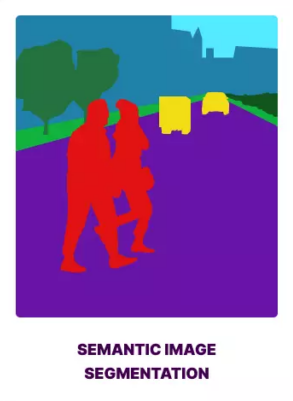
\includegraphics[width=2.5cm]{seg.png}  
\end{minipage}

\end{figure}

\begin{figure}[h]
\centering

\begin{minipage}{0.7\textwidth}
\begin{itemize}
    \item \textbf{la segmentation panoptique} : 
    Il s'agit de la méthode la plus performante, qui sépare les objets en catégories et en instances distinctes. Elle serait plus précise car elle permettrait de segmenter directement chaque astrocyte de l'image, et repérer plus simplement ses structures.
    Le soucis c'est qu'elle nécessite beaucoup de données et a un temps plus long de traitement. 
    Par ailleurs, elle nécessite une intervention humaine pour choisir quelles sous parties sont connectées (il faudra réunir manuellement les structures détectées).
\end{itemize}
\end{minipage}
\hfill
\begin{minipage}{0.27\textwidth}
     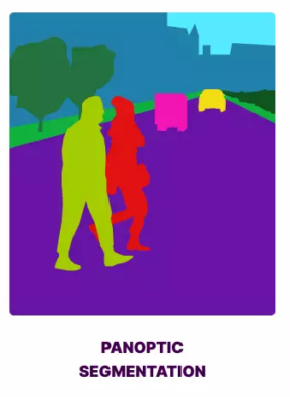
\includegraphics[width=2.5cm]{pano.png}  
\end{minipage}

\end{figure}

Par ailleurs, \textbf{la segmentation panoptique de parties}  est celle qui permettrait un traitement pleinement automatisé des données de chaque astrocyte . Au lieu de recomposer manuellement un astrocyte à partir de ses composants segmentés, ou d'avoir des données groupées par catégorie de structures, cette segmentation est capable d’identifier chaque élément et comprendre ses parties, elle pourrait donc passer à l'étape de l'analyse des mitochondries sans friction, séparément pour chaque astrocyte.\\

Cependant, il est important de savoir que pour une amélioration mineure en terme de simplification d'utilisation, les besoin techniques augmentent fortement : au delà de devoir résoudre le problème des structures spongiformes qui se superposent, l'analyse et demanderait de passer à un modèle d'U-Net avancé qui serait plus lourd à faire tourner (\ref{fig:img mask}). 
\begin{figure}[!h]
\centering
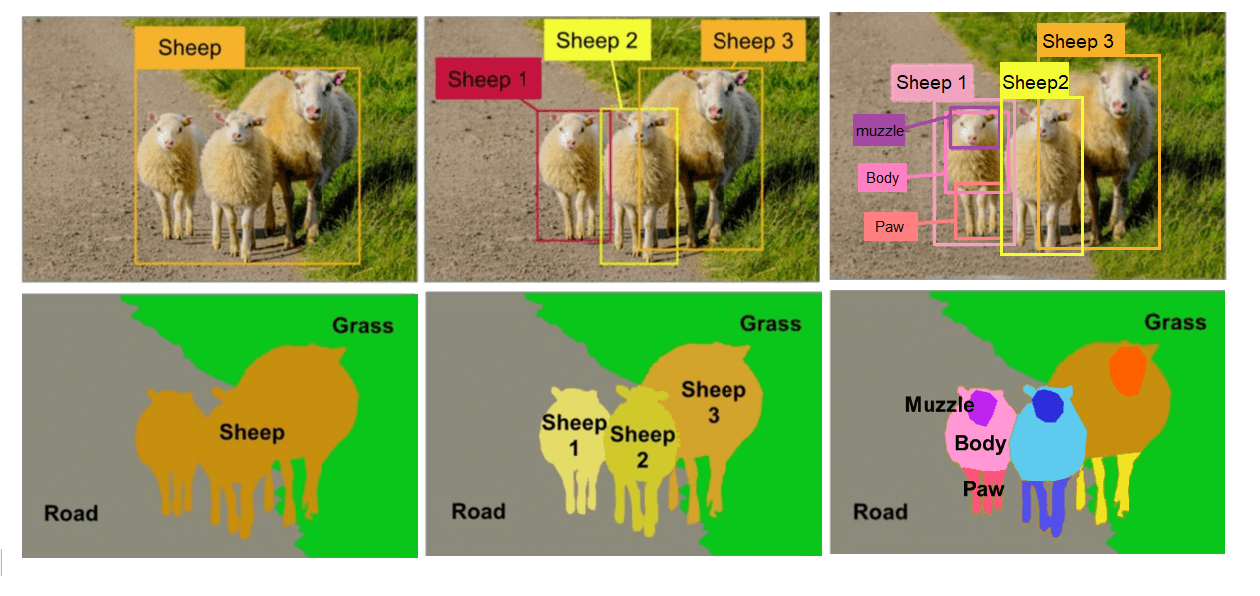
\includegraphics[width=0.75\linewidth]{segmentation.png}
\caption{\label{fig:seg part}Illustration des types de segmentation (sémantique/ panoptique/panoptique de parties)}
\end{figure}
\\
On choisi un programme de segmentation sémantique car nos données disponibles ne sont pas annotées au delà des compartiments (\ref{fig:img soma}/\ref{fig:mask process}/\ref{fig:img spong}) et qu'on peu de données.
Pour ce cas, la segmentation sémantique suffit à localiser les parties où sont les mitochondries, pour analyser leur réseau par la suite. \\

\subsection{l'analyse avec U-Net }

\subsubsection{fonctionnement de U-Net}
U-Net est un réseau de neurones créé pour faire de l'analyse d'images, en particulier de la segmentation sémantique. \\
Dans les réseaux de neurones artificiels, les "neurones" sont des valeurs entre 0 et 1, qui s'organisent sur plusieurs couches connectées dont les valeurs dépendent des couches de "neurones" précédentes. La première couche de neurones correspond aux valeurs des pixels de l'image, la dernière est le résultat appliqué à l'image, celles qui sont entre les deux correspondent au calcul des paramètres. 
Pour influencer la couche suivante, les neurones ont un "poids" qui donne l'importance de chaque pixel. 


Il a 4 étapes, l'encodeur qui extrait des informations via des convolutions, le goulot d'étranglement où toute l'information est condensée, le décodeur qui tente de reproduire l'image à l'aide de "up-convolutions" qui sont dans le texte et les connexions qui vont connecter les informations du bloc de l'encodeur correspondante.  


A la fin de chaque tour de U-Net, le réseau sort un masque (avec une fonction sigmoïde), qui quantifie sa capacité à segmenter l'objet. 
Avec la fonction de perte, le réseau est puni si il fait une erreur ou alors récompensé. 
Le réseau recalcule les paramètres à changer, puis à l'aide d'un optimiseur (Adam) il corrige l'erreur (petit à petit) , recommence jusqu'à optimiser la fonction de perte. 

\subsubsection{types de U-Net}

U-Net multi-classes 
affecte chaque pixel à une classe 
-efficace 
-compétition entre les classes : plus de contexte

(les classes peu présentes sont moins bien apprises) 

U Net binaire 
chaque modèle fait une sortie indépendante 

lorsque un pixel appartient à plusieurs classes le modèle est plus performant. 
Aussi le modèle permet de mieux supprimer les bruits. 

\subsubsection{paramètres de U-Net}

Dice loss
mesure du recouvrement entre la vérité terrain et la prédiction du modèle. 
évite de s'entraîner sur le fond

Focal loss 
améliore la crossentropy : ignore le fond et force le réseau a travailler sur les pixels plus complexes. (modification du gamma

Pondération des classes 
: dit à quel point faire une errreur est important. 
Souvent le poid est proportionnel à la fréquence des lcasses, mais si le poid est trop grand on a des faux positifs 

oversampling
Si certains objets sont rarement présents  Cause des problèmes de mémorisation et d'overfitting


Deep supervision 


\subsection{conception du programme}

On souhaite obtenir une segmentation sémantique (\ref{fig:seg part}) de notre astrocyte. 

Pour le réaliser, on va tester plusieurs approches,  mais aussi proposer une segmentation de par parties (pour le cytosol, le soma, les processus et les structures spongiformes).
L'idée n'est pas uniquement de proposer plusieurs options, mais d'entraîner les modèles qui fonctionnent mal qu'on souhaite utiliser avec les résultats de ceux qui fonctionnent le mieux.


\subsection{pipeline de U-Net}

- U-Net sur le cytosol : supprimer le fond 


- détecter et supprimer les noyaux intrus 
- détecter et les processus intrus 
- 




\section{Paramètres du programme}
Nos paramètres vont dépendre de l'anatomie des astrocytes mais aussi de la manière dont les masques ont été réalisés : dans les masques du soma des processus et des structures spongiformes , les chercheurs ont fait le choix de garder uniquement les astrocytes les plus "complets" dont les parties sont totalement, ou quasi totalement présentes dans les 3 dimensions, ce qui a pour conséquence de rendre plus complexe le choix des critères morphologiques qui vont identifier les astrocytes d'intérêt tout en discriminant les autres et va impacter la capacité du programme à comprendre la différence entre les bons et les mauvais objets.

On cherche donc des solutions pour parvenir à utiliser les masques disponibles. 

Par ailleurs les chercheurs ont considéré comme background les images qu'ils n'arrivaient pas à segmenter car inexploitables: à moins d'entraîner un modèle qui cherche les régions ou la segmentation est trop complexe, il faudra supprimer ces images du jeu de données.



\subsection{caractères des parties de l'astrocyte}
Afin de pouvoir au mieux segmenter les parties, on cherche des spécificités qu'on va forcer le programme à intégrer afin qu'il les repère malgré leur complexité.

\begin{figure}[htbp]
    \centering
    % Première image 
    \begin{minipage}{0.23\textwidth}
        \centering
        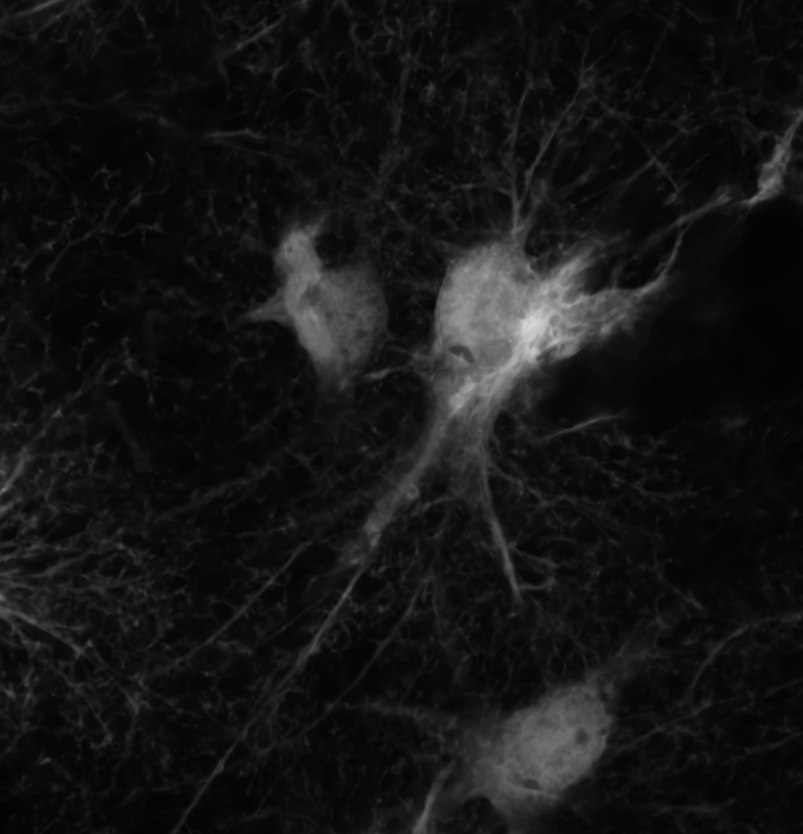
\includegraphics[width=\textwidth]{img origin.png}
        \caption{Image type avec plusieurs astrocytes}
        \label{fig:img origin}
    \end{minipage}\hfill
    % Deuxième image (33 data 7) 
    \begin{minipage}{0.23\textwidth}
        \centering
        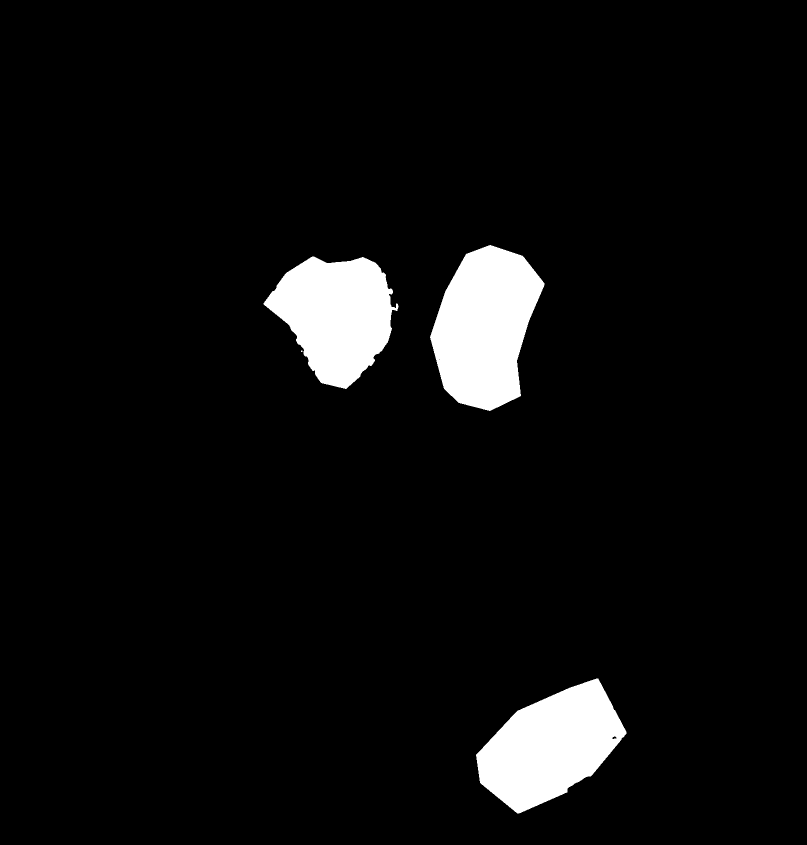
\includegraphics[width=\textwidth]{img mask.png}
        \caption{Masque type des somas}
        \label{fig:img soma}
    \end{minipage}\hfill
       % Troisième image(figure 33 data 7) 
    \begin{minipage}{0.23\textwidth}
        \centering
        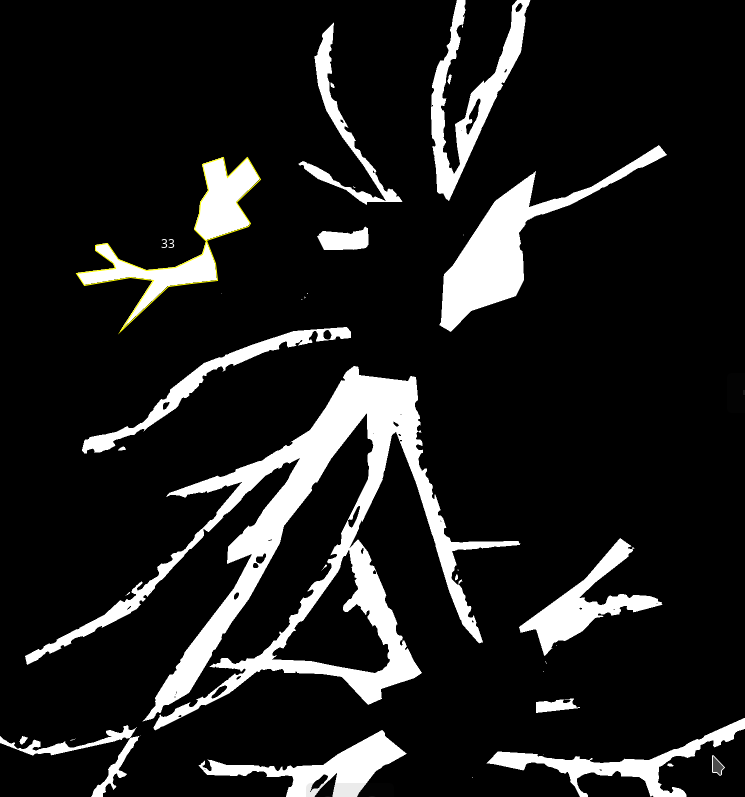
\includegraphics[width=\textwidth]{img mask Process.png}
        \caption{\label{fig:mask process}Masque type des processus.}
    \end{minipage}\hfill
      % Quatrième image(figure 31 data 7) 
    \begin{minipage}{0.23\textwidth}
        \centering
        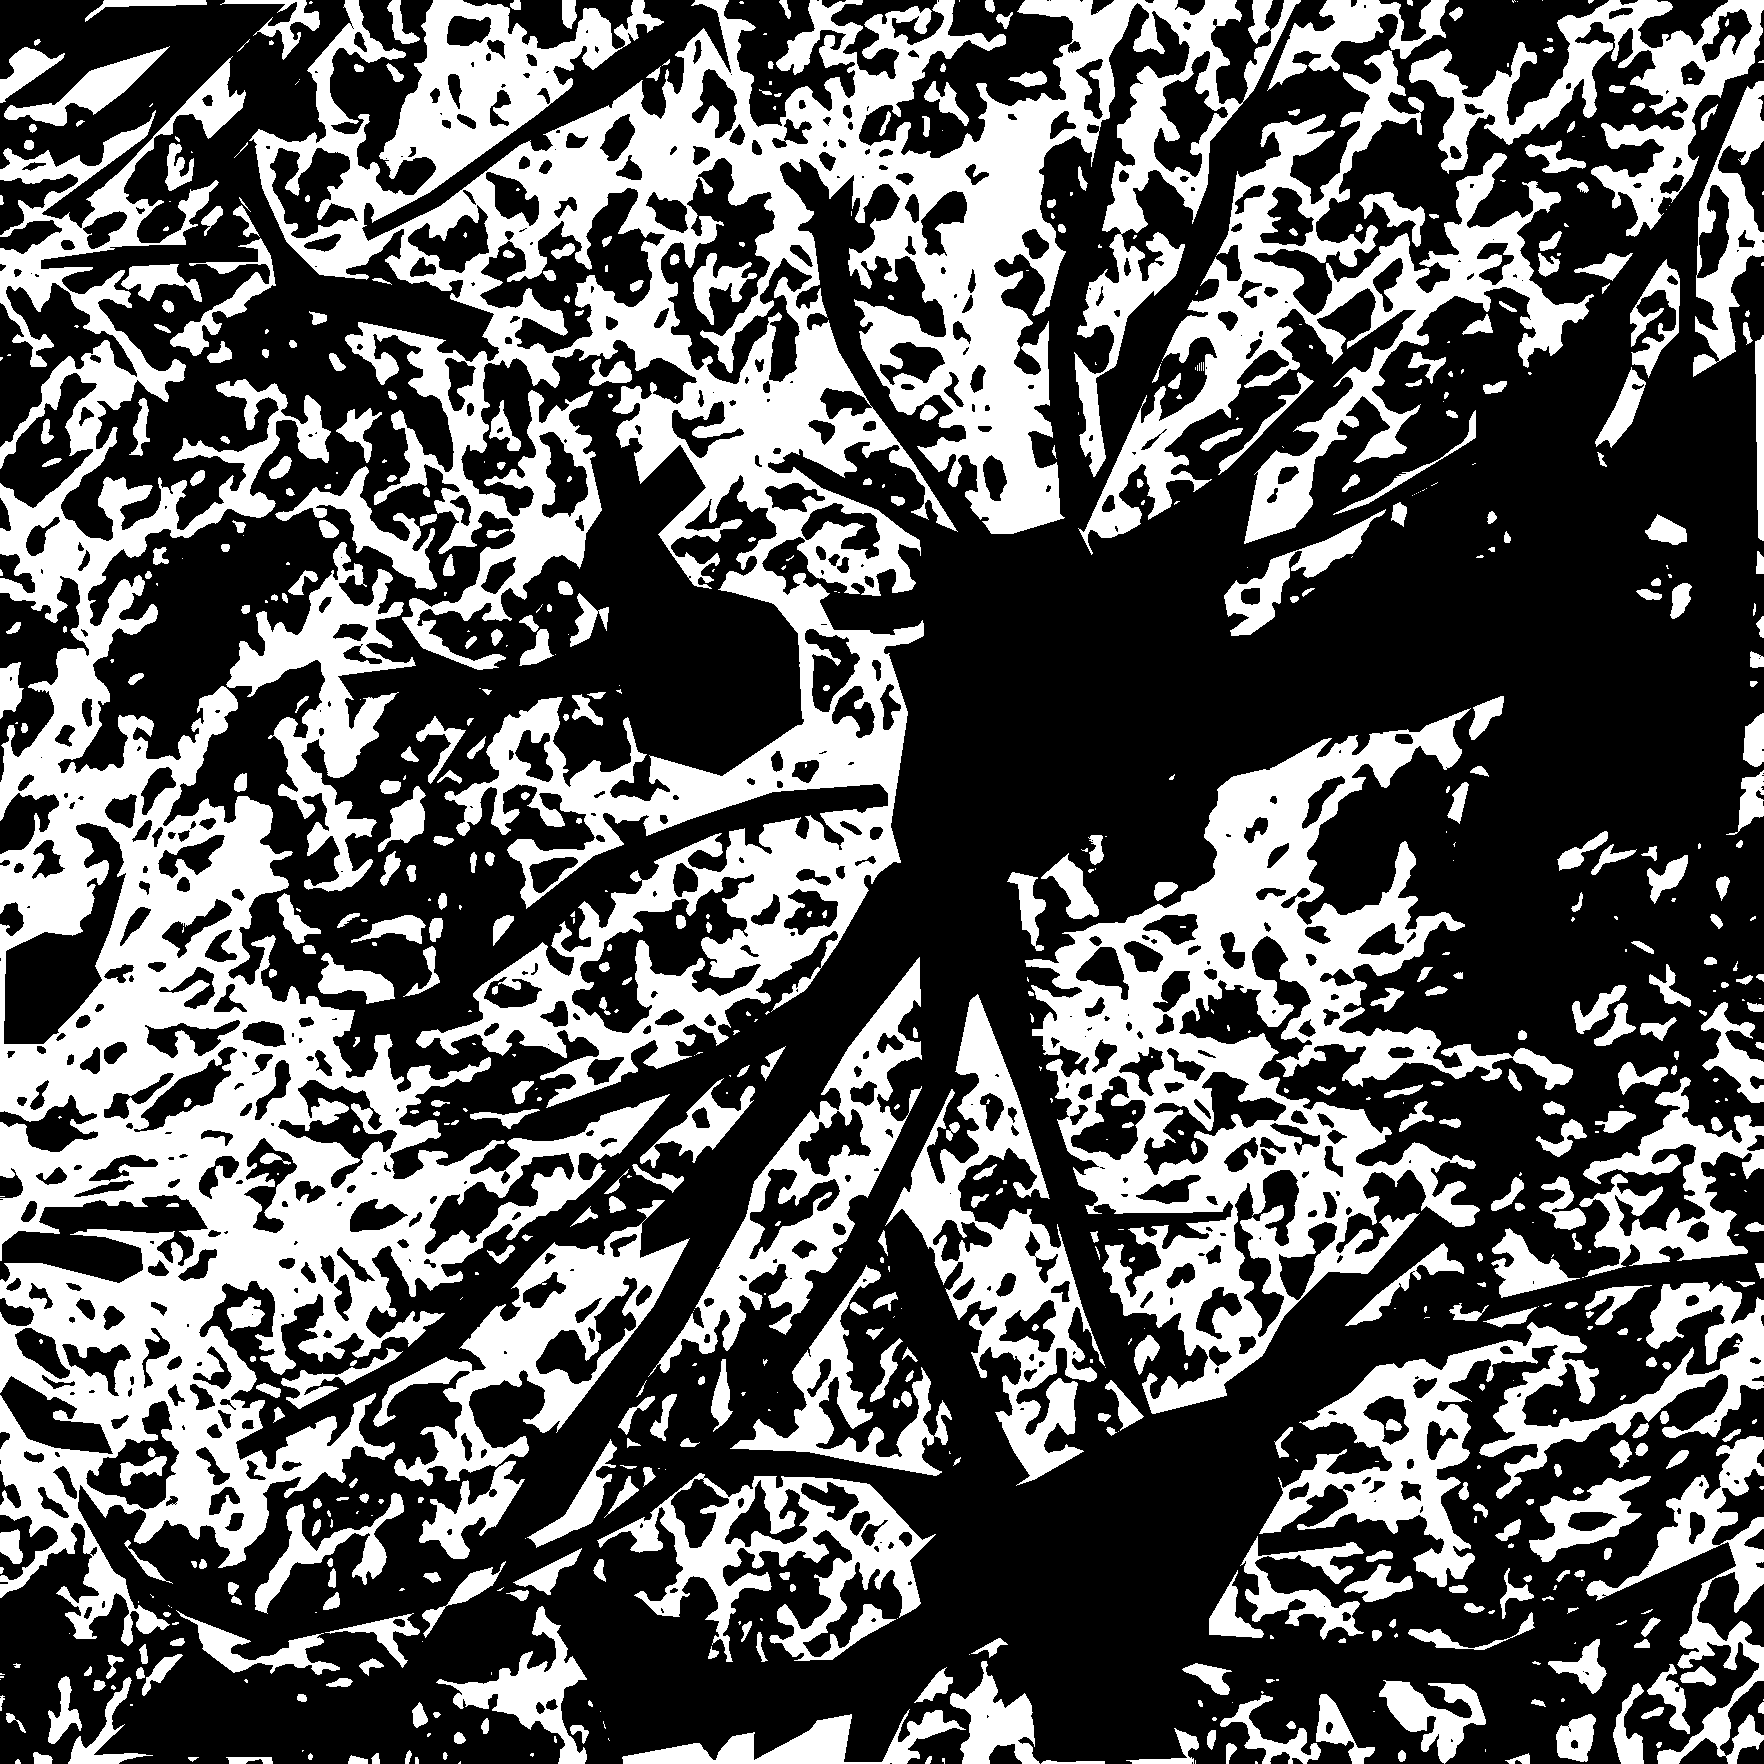
\includegraphics[width=\textwidth]{spongi.png}
        \caption{Masque type des structures spongiformes}
        \label{fig:img spong}
    \end{minipage}
\end{figure}

\subsubsection{Les noyaux}

Pour le repérer, on va inciter le programme à ce concentrer sur des caractères qui lui sont spécifiques : 
\begin{itemize}[label=$\circ$]
    \item sa taille (elle représente environ 5\% de l'image ) 
    \item sa forme (elle est plutôt ronde, et a un rayon maximum) 
    \item son intensité (qui est la plus forte dans l'image d'origine) 
    \item le nombre (on a difficilement plus de 7 astrocytes dans nos images)
\end{itemize}

Le caractère le plus délicat est le point de contact et l'orientation des processus. Car les processus partent toujours du noyau, leur position est déterminante pour le localiser. Néanmoins c'est aussi une source d'erreurs dans le cas ou les processus se superposent, et son efficacité dépend de la capacité du modèle à détecter au mieux les processus. 

\subsubsection{Les processus}

La difficulté pour les processus c'est que les processus de différents astrocytes peuvent se chevaucher, de plus, les processus ne sont pas segmentés individuellement, on doit donc trouver les caractères spécifiques au "réseau de processus". 
On peut repérer : 
- la connectivité (connexions aux noyau et aux structures spongiformes) 
- une arborescence de "tronc"
- des diamètres de taille décroissante.
- un diamètre minimum
- l'intensité 

Dans nos données, à certains moment les chercheurs font le choix d'ignorer les processus des astrocytes "intrus", sans une segmentation de partie (\ref{fig:seg part}) il n'est pas possible de supprimer les processus des astrocytes qui ne nous intéressent pas sans les considérer comme n'étant pas des processus, ce qui rend la tache du choix des caractères plus complexe, d'autant plus que notre jeu de données peut parfois choisir de prendre qu'un seul astrocyte car il est "complet" et parfois délimiter plusieurs astrocytes.

\subsubsection{Les structures spongiformes}
Comme elle est difficilement obtenue, la partie structure spongiforme correspond en réalité au masque du cytosol, moins les masques du soma et des processus. 
Ce masque possède donc les parties des astrocytes "intrus".

Ceci complexifie les paramètres qu'on peut utiliser pour définir les structures spongiformes :
les caractères spécifiques comme
leur faible intensité,
la forme en arborescence,
les liens avec le soma et les processus,
ne sont plus exploitables sur certaines piles de données. 


Par ailleurs, quand les somas, et les processus intrus sont supprimés, 

\begin{figure}[htbp]
    \centering
     %  image(figure 35 data 8) 
    \begin{minipage}{0.33\textwidth}
        \centering
    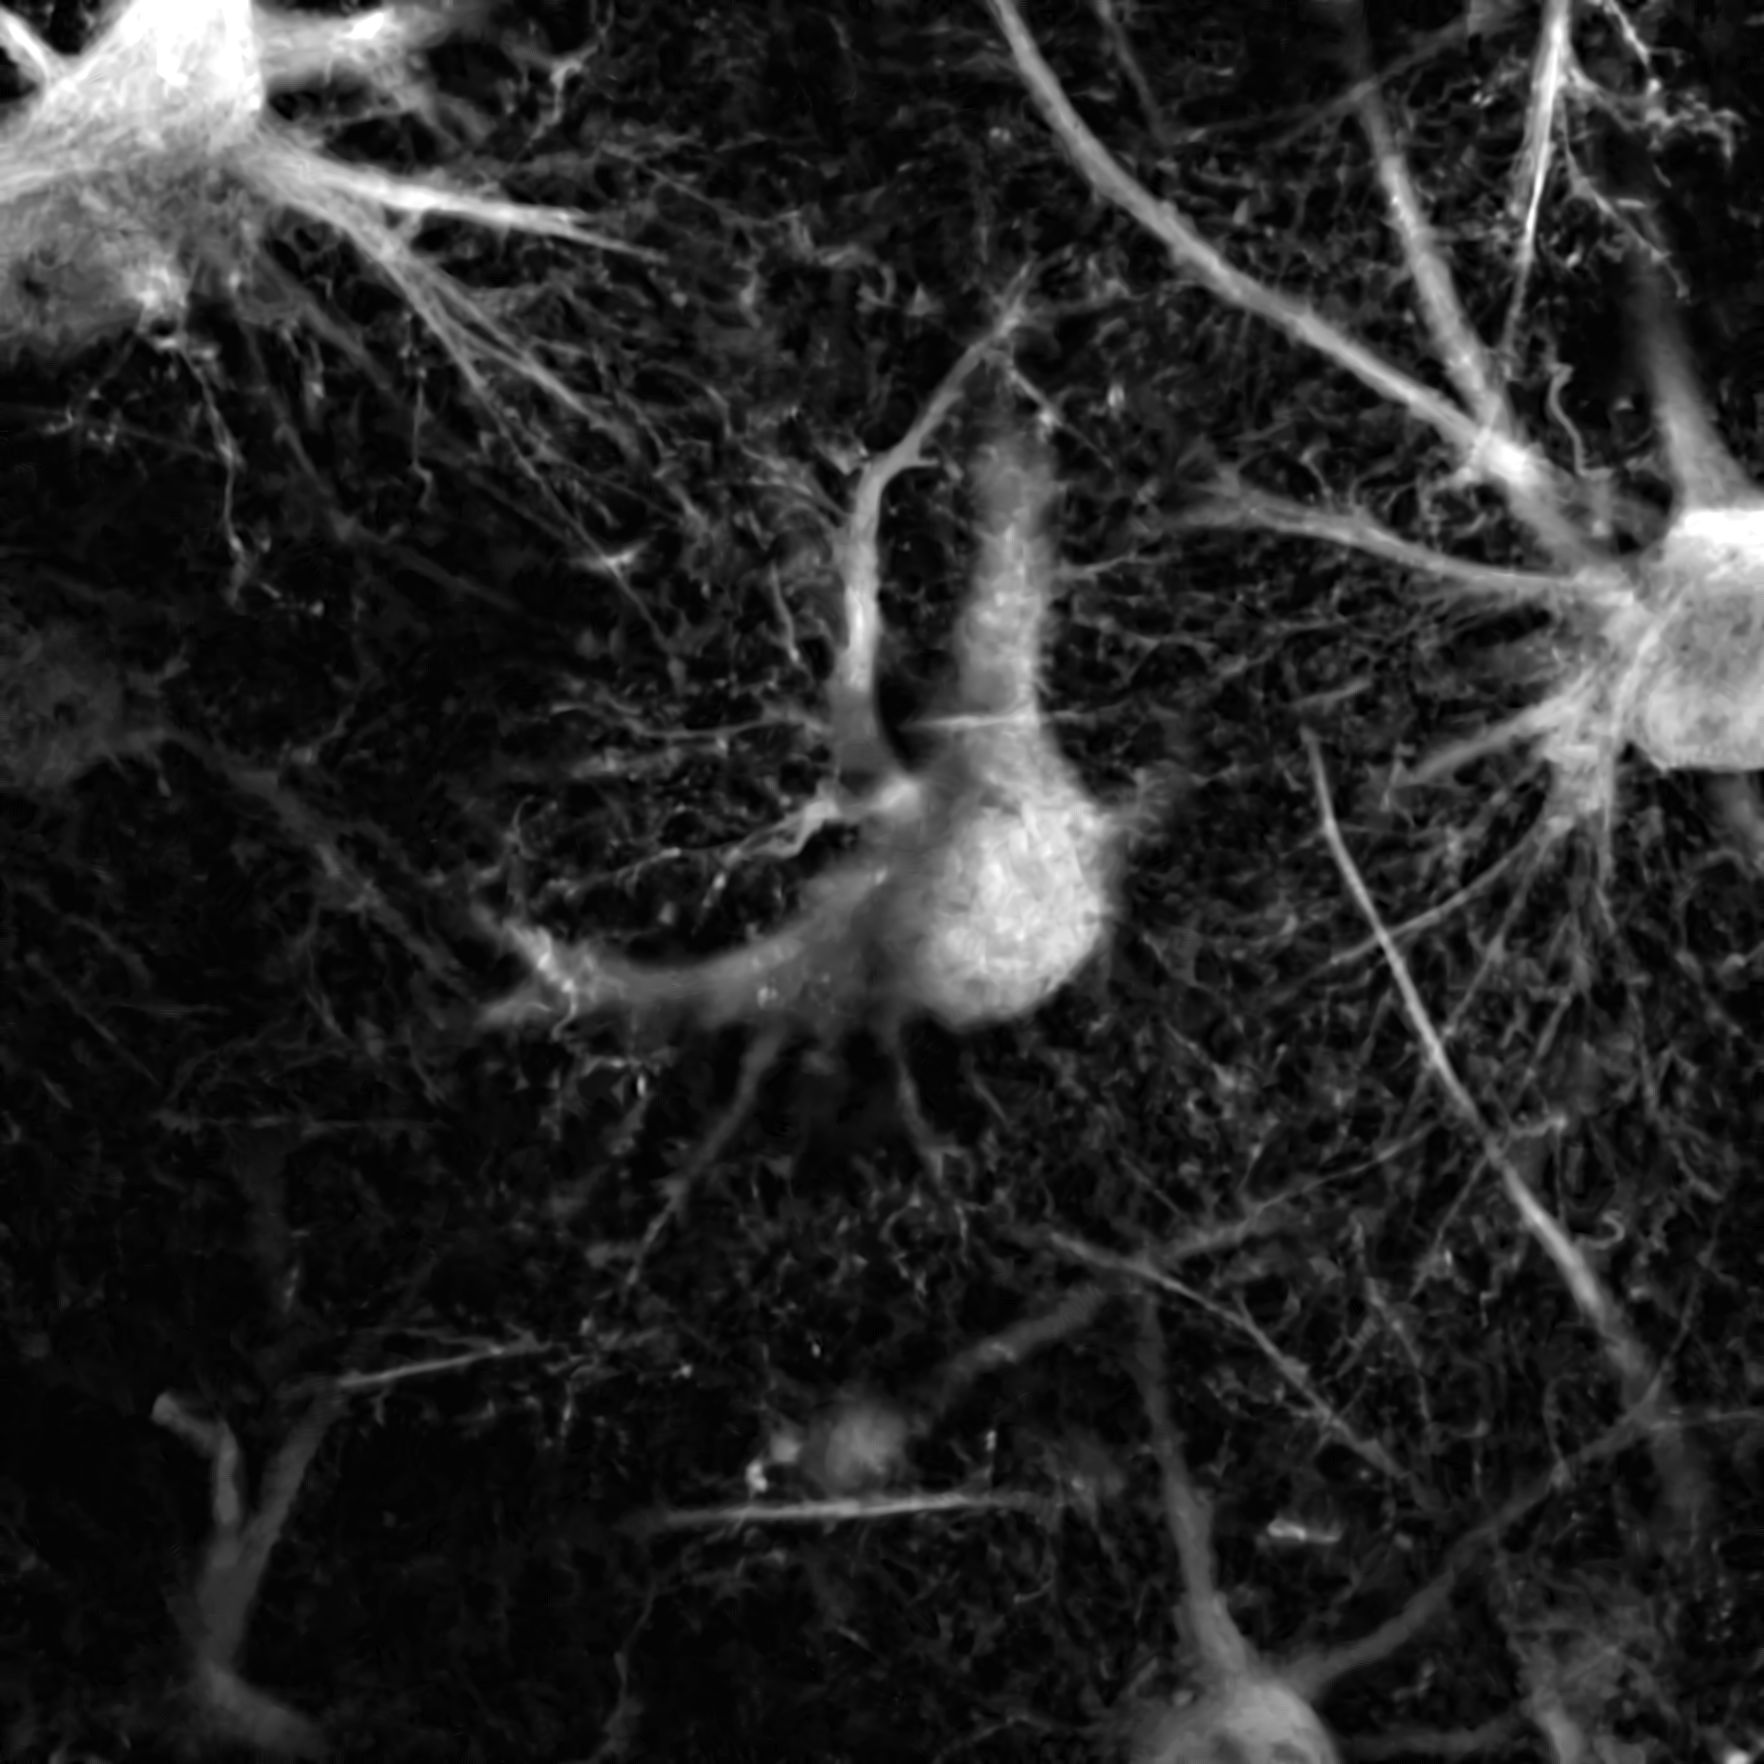
\includegraphics[width=\textwidth]{bad spongi original.png}
        \caption{\label{fig:bspong}Image originale.}
    \end{minipage}\hspace{0.7cm}
      % Quatrième image(figure 35 data 8) 
    \begin{minipage}{0.33\textwidth}
        \centering
    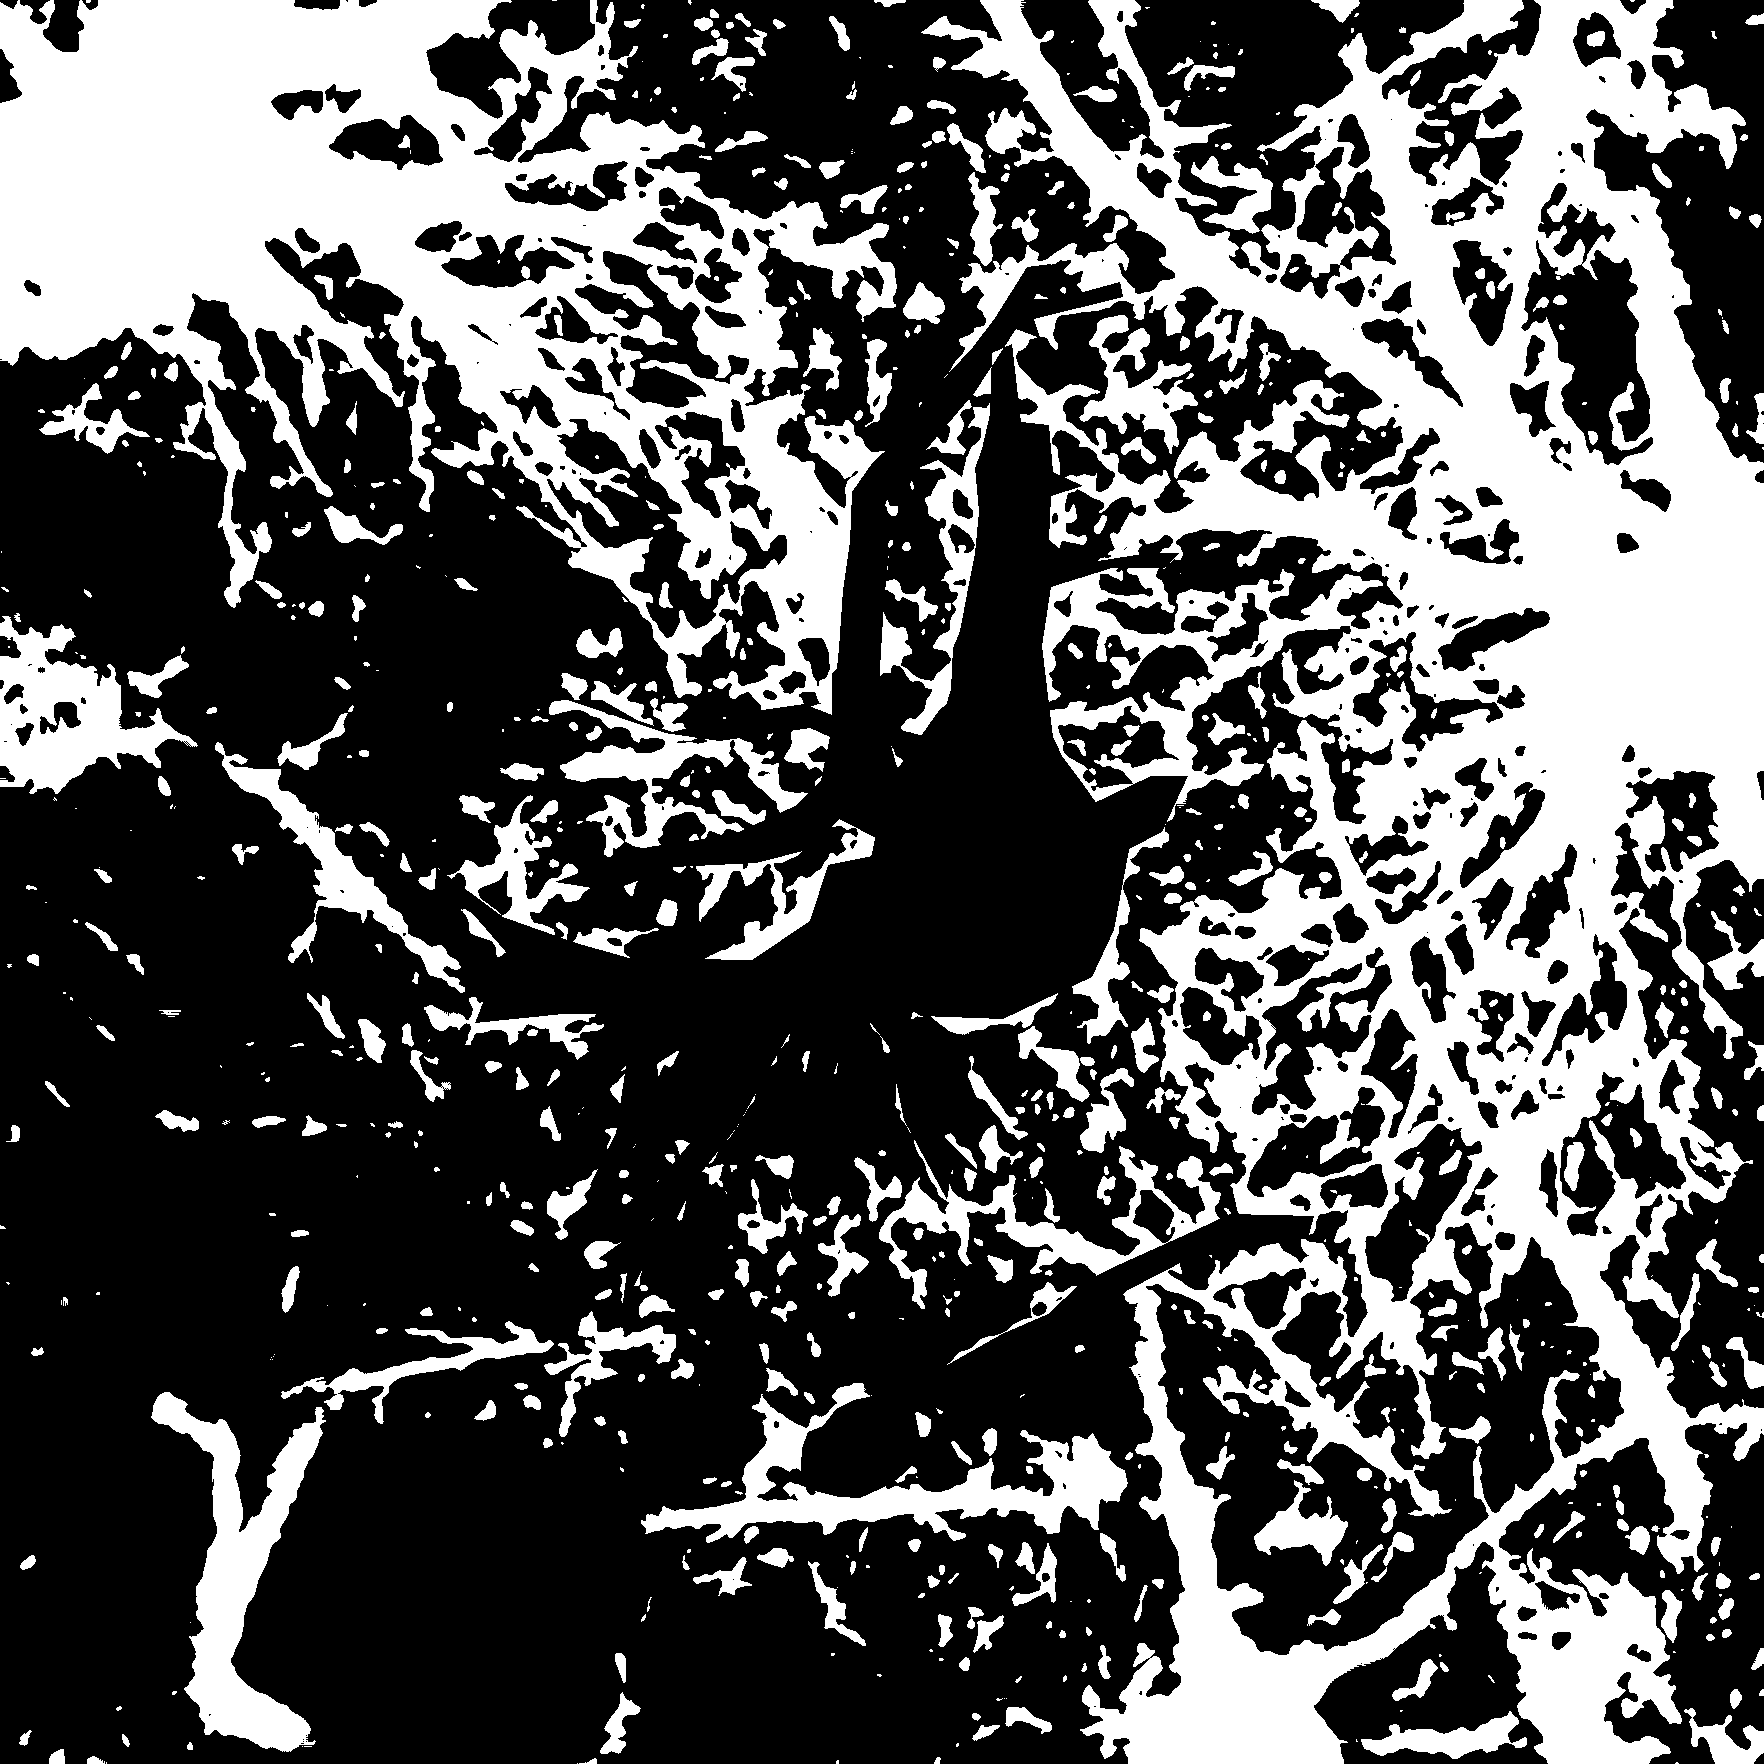
\includegraphics[width=\textwidth]{bad spongi.png}
        \caption{Masque des chercheurs}
        \label{fig:bspongm}
    \end{minipage}
\end{figure}

\subsection{caractères du jeu de données}
les chercheurs font un certain nombre de biais dans leur choix sur les astrocytes d'intérêt, certains sont identifiables et peuvent nous aider à améliorer la segmentation. 

\subsubsection{la position des astrocytes}

Les astrocytes d'intérêt choisis sont généralement présent dans les 3 dimensions (pour visualiser la distribution des mitochondries dans tous les compartiments) et leurs noyaux sont souvent plus larges au centre des piles d'images. 
En indiquant de les rechercher plutôt vers le centre de la pile, on peut utiliser à notre avantage le choix des chercheurs. 

\subsubsection{la forme des segmentations}
Les parties sont souvent segmentées à l'aide de traits droits pour accélérer le processus manuel, ce qui peut causer des défauts de délimitation qui perturbent la reconnaissance.
De plus les chercheurs n'accordent que peu d'importance à la délimitation très précise des compartiments, qui ont eux même une définition biologique peu précise. 
Ce qui nous permet de pouvoir dire au programme de ne pas accorder trop d'importance aux erreurs, si elles sont à quelques pixels des parties segmentées du masque, ce qui limite les perturbations et ne diminue pas les résultats.  



\begin{figure}
\centering
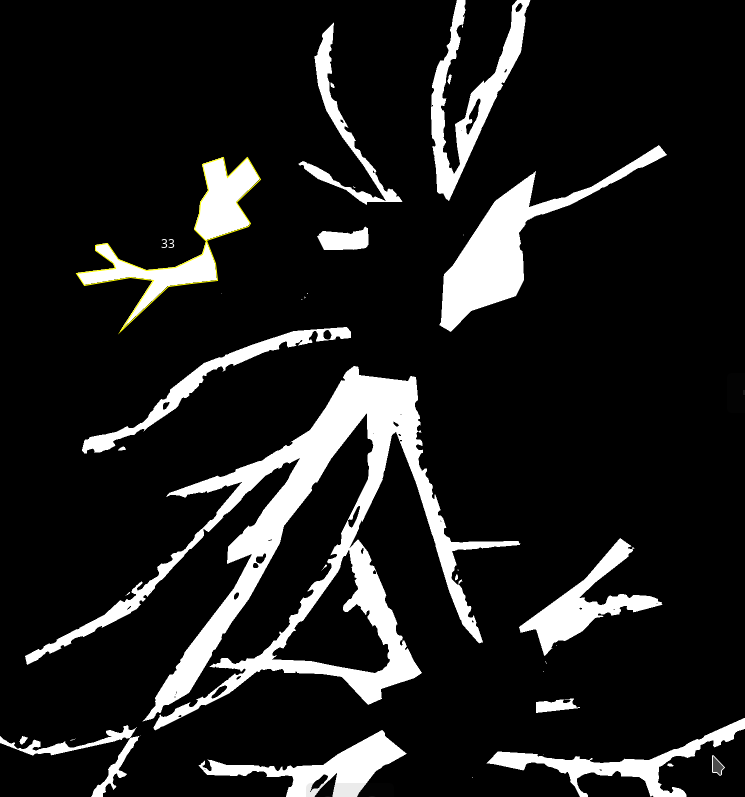
\includegraphics[width=0.25\linewidth]{img mask Process.png}
\caption{\label{fig:mask process2}Image type des processus.}
\end{figure}


 Augmentation de données 

- tourner ... les données 

-tourner dans les 3 dimensions 

- déformations élastiques du jeu de données




Toucher au unet 

- moins de convolutions par bloc (aucun détail) : évite le sur apprentissage 
- ne pas prendre en compte des connexions spécifiques (repérer des structures spécifiques)



Toucher aux options 

- generalized Dice loss : 
si une classe n'est pas beaucoup présente on va lui accorder plus d'importance



\end{document}
